\chapter{Risultati sperimentali}
\label{chap:risultati}
\vspace{1cm}
Questo capitolo illustra i risultati del lavoro, descrivendo
il procedimento effettuato per validare la metodologia proposta
in questa tesi.

La sezione \ref{sec:ambienteTest} descrive l'ambiente e le
modalit\`a con cui sono stati ricavati i risultati contenuti
in questo capitolo.

La sezione \ref{sec:risultatiEsplorazione} mostra i grafici relativi
ai risultati ottenuti eseguendo l'algoritmo di esplorazione.
Vengono descritti i grafici dello speedup ottenuto
confrontando un'esecuzione puramente in software con la possibilit\`a
di utilizzare anche risorse hardware, riconfigurabili o meno, allo
scopo di dimostrare come MapR permetta di valutare in maniera efficace
quando l'utilizzo della riconfigurazione parziale dinamica porti benefici al
tempo di esecuzione dell'applicazione. Vengono descritti grafici relativi
al mapping dei task, numero di core e area utilizzata, oltre a un confronto
dell'applicazione dopo l'esecuzione effettiva su un dispositivo.

\newpage

\section{Ambiente di test}
\label{sec:ambienteTest}

La metodologia proposta \`e stata valutata mediante l'esecuzione
dell'algoritmo di esplorazione su un insieme di task graph,
con diverse architetture di riferimento.


\begin{figure}[t]
  \begin{center}
    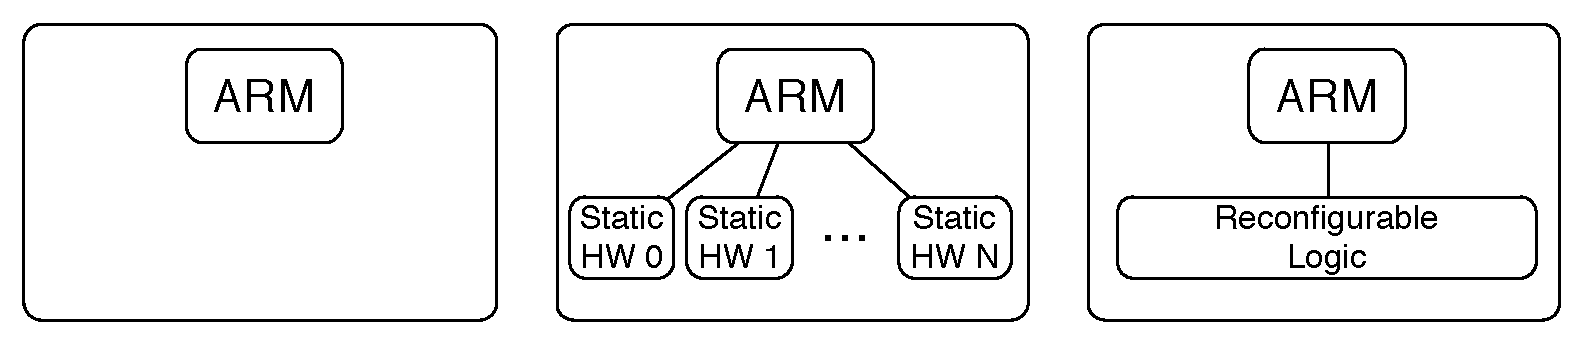
\includegraphics[width=0.7\textwidth]{./capitoli/figure/cap6/templates.pdf}
    \caption{Architetture di riferimento utilizzate per i test su benchmark sintetici.}
    \label{fig:architettureTestSintetici}
  \end{center}
\end{figure}

Le architetture utilizzate
sono rappresentate in figura \ref{fig:architettureTestSintetici}. La prima \`e un'architettura puramente
software che serve da baseline; in questo caso il tool non pu\`o utilizzare risorse hardware.
La seconda \`e caratterizzata anche da processing element hardware \emph{statici}, quindi MapR non pu\`o
sfruttare le potenzialit\`a della riconfigurazione, tuttavia \`e possibile mappare task in hardware;
il numero massimo di core utilizzabili \`e specificabile dal designer, in questi test
\`e stato impostato al numero massimo di task usati negli esperimenti.
L'ultima architettura \`e caratterizzata dalla presenza di una o pi\`u aree riconfigurabili, in questo
caso la riconfigurazione parziale dinamica pu\`o essere sfruttata da MapR.


I task graph usati come benchmark per la validazione del funzionamento di
\mbox{MapR} sono stati generati utilizzando \ac{TGFF} \cite{tgff}, uno strumento per
la generazione di task graph pseudo-casuali ampiamente utilizzato.
I task graph cos\`i generati differiscono nel numero di nodi (task) e di implementazioni
disponibili per ciascun task. Ogni implementazione \`e caratterizzata dai propri requisiti
di area e tempo di esecuzione. Per effettuare i test sui benchmark \`e stato generato un insieme di 25 task graph da
10, 20, 30, 40, 50 nodi (5 istanze per ogni numero di nodi). I parametri pi\`u importanti specificati
nel file di configurazione di \ac{TGFF} per la generazione dei task graph sono indicati nella tabella
\ref{tab:parametriTGFF}.

\begin{table}[t]
  \begin{center}
  \begin{tabular}{|c|c|c|}
    \hline
    \textbf{Nome} & \textbf{Descrizione} & \textbf{Valore}\\
    \hline
    \emph{task\_cnt} & Numero task & Da 10 a 50\\
    \hline
    \emph{task\_degree} & Massimo numero di archi per task & 4\\
    \hline
    \emph{tg\_cnt} & Numero di task graph da generare & 1\\
    \hline
  \end{tabular}
  \caption{Parametri usati per la generazione di task graph con \acs{TGFF}.}
  \label{tab:parametriTGFF}
\end{center}
\end{table}


\section{Risultati dell'esplorazione}
\label{sec:risultatiEsplorazione}
Dopo aver generato i task graph con le modalit\`a descritte nella precedente
sezione, l'esplorazione \`e stata eseguita e i makespan relativi alla migliore soluzione
trovata nell'esplorazione corrente sono stati salvati per tutte le architetture.
La funzione obiettivo dell'algoritmo di esplorazione utilizzata per questi esperimenti
\`e basata solamente sulla stima del makespan calcolata dallo scheduler descritta nel
capitolo \ref{chap:approccio}.

I parametri relativi all'algoritmo di esplorazione sono indicati nella tabella \ref{tab:parametriACO}.
Il numero di formiche sopravvissute si riferisce a quante soluzioni tra quelle calcolate dalla generazione
vengono utilizzate per il rinforzo della matrice dei feromoni. I parametri $\alpha$ e $\beta$
rappresentano i pesi dati alle euristiche locali e globali dei task e dei possibili mapping.


\begin{table}[t]
  \begin{center}
    \begin{tabular}{|c|c|}
      \hline
      \textbf{Nome} & \textbf{Valore}\\
      \hline
      Numero iterazioni & 100\\
      \hline
      Formiche per generazione & 20\\
      \hline
      Formiche sopravvissute & 2\\
      \hline
      Massimo incremento area \% & $25\%$\\
      \hline
      $\alpha_t$ & $0,9$\\
      \hline
      $\beta_t$ & $0,1$\\
      \hline
      $\alpha_{pi}$ & $0,9$\\
      \hline
      $\beta_{pi}$ & $0,1$\\
      \hline
    \end{tabular}
    \caption{Parametri usati per l'algoritmo di esplorazione.}
    \label{tab:parametriACO}
  \end{center}
\end{table}

\begin{figure}[t]
 \begin{center}
  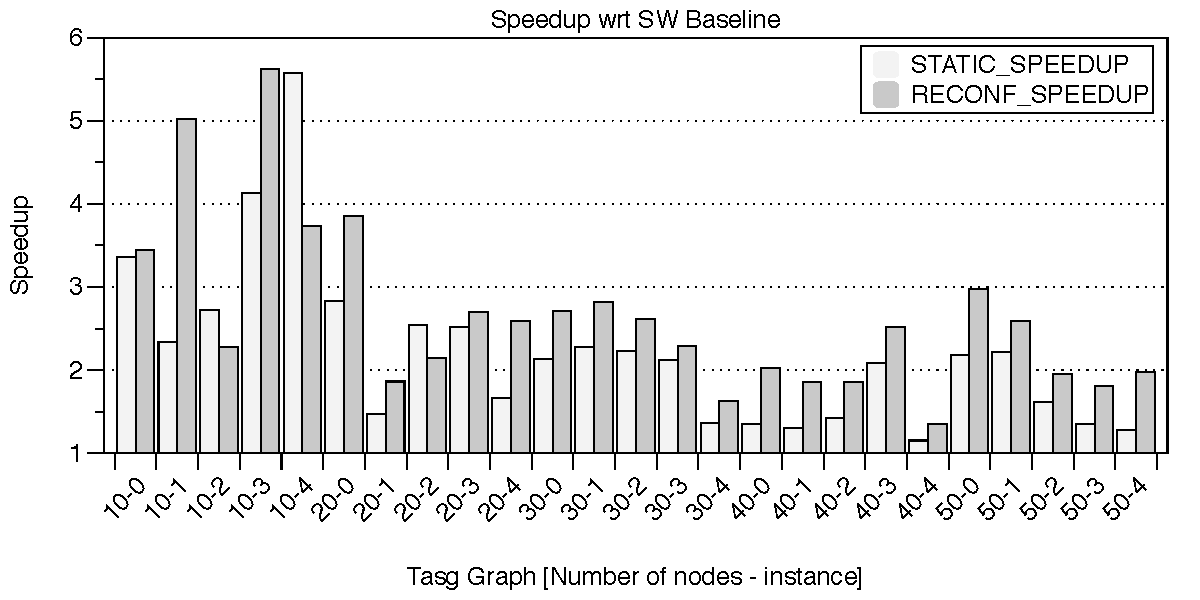
\includegraphics[width=\textwidth]{./capitoli/figure/cap6/FPL_makespan.pdf}
  \caption{Speedup dell'architettura statica e riconfigurabile rispetto alla
  baseline software.}
  \label{fig:speedupBaseline}
 \end{center}
\end{figure}

\subsection{Speedup rispetto a baseline software}
La figura \ref{fig:speedupBaseline} rappresenta lo speedup ottenuto utilizzando
le architetture hardware statica e riconfigurabile rispetto alla baseline
con implementazioni esclusivamente software, per tutti i task graph oggetto
dell'esplorazione. Si pu\`o vedere che per tutti i task graph MapR riesce ad
avere uno speedup rispetto alla baseline, che varia da circa $2\text{x}$ per istanze con
un elevato numero di nodi, fino a $5,5\text{x}$ con istanze pi\`u piccole. La differenza
tra gli speedup rappresentati in figura \ref{fig:speedupBaseline} \`e dovuta al fatto che,
pur avendo lo stesso numero di nodi, le istanze in realt\`a hanno topologie e tempi di
esecuzione potenzialmente molto diversi: questo fattore influisce sulla lunghezza dello schedule
al termine dell'esplorazione.
Inoltre, si pu\`o vedere dalla figura che, con il crescere della dimensione dei task graph e
conseguente scarsit\`a di risorse hardware, MapR riesce a sfruttare efficacemente la riconfigurazione
parziale dinamica e a ottenere risultati migliori impiegando l'architettura riconfigurabile.

\begin{figure}[t]
 \begin{center}
  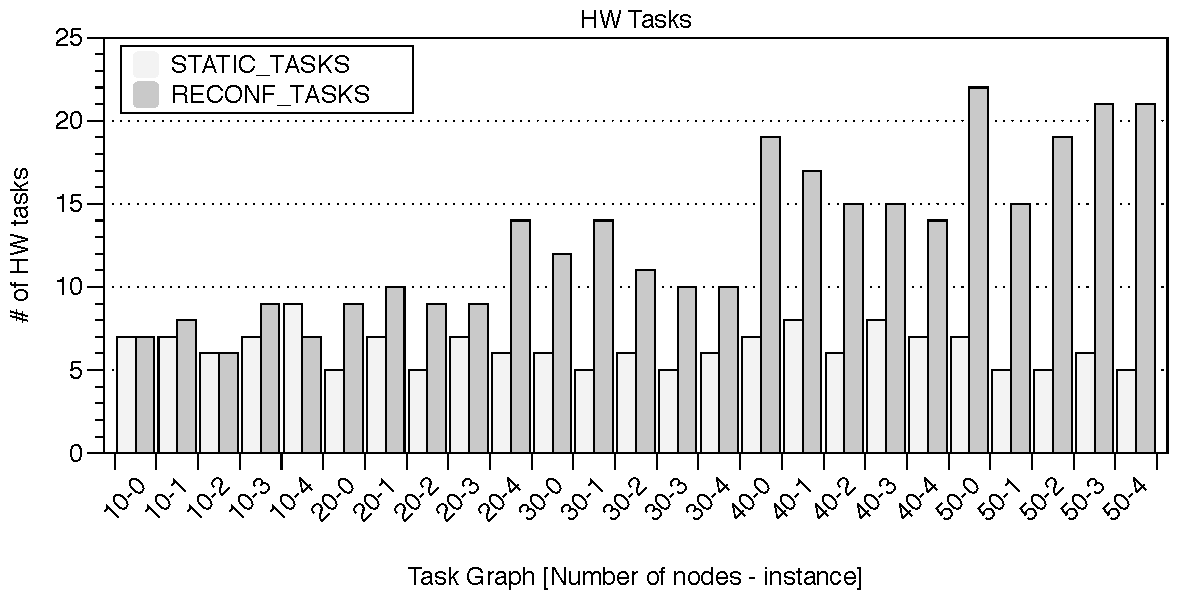
\includegraphics[width=\textwidth]{./capitoli/figure/cap6/FPL_HWtasks.pdf}
  \caption[Numero di task implementati in hardware.]{Numero di task implementati in hardware; dati relativi ai due template architetturali
  che possono utilizzare la logica riconfigurabile.}
  \label{fig:hardwareTask}
 \end{center}
\end{figure}

\subsection{Dati relativi al mapping dei task}
La figura \ref{fig:hardwareTask} rappresenta il numero di task che sono stati mappati
dall'algoritmo di esplorazione su logica riconfigurabile.
In questo caso sono stati considerati i due template architetturali che permettono
l'utilizzo della logica riconfigurabile, dando piena libert\`a
a MapR di decidere quanti e quali task mappare su core statici o regioni riconfigurabili del dispositivo.
I risultati confermano quanto anticipato nel paragrafo precedente: al crescere del numero di
task quando le risorse hardware sono scarse, in ottica di minimizzazione del makespan, la possibilit\`a di sfruttare
la riconfigurazione parziale permette a MapR di spostare
in hardware un maggior numero di task, sfruttando meglio l'area a disposizione.

Ad esempio, considerando l'ultimo task graph (50-4), MapR \`e riuscito ad ottenere uno speedup di
$1,2\text{x}$ nel caso statico implementando 5 task in hardware; avendo a disposizione l'architettura
riconfigurabile, lo speedup ottenuto \`e stato di $2\text{x}$ rispetto alla baseline software,
spostando 21 task in hardware.

\begin{figure}[t]
 \begin{center}
  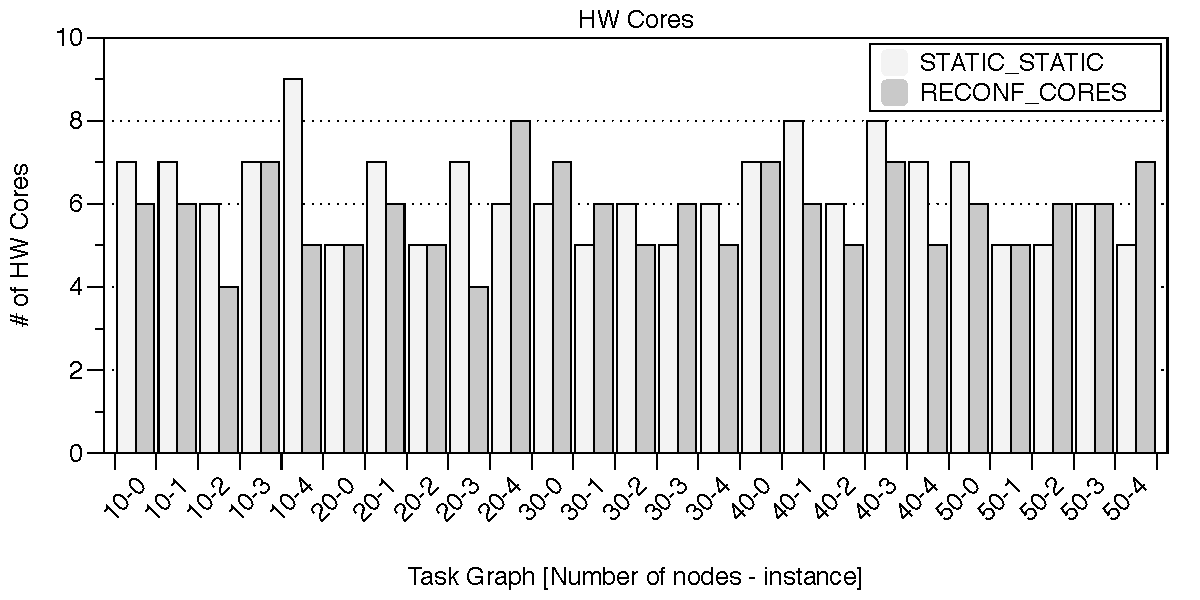
\includegraphics[width=\textwidth]{./capitoli/figure/cap6/FPL_HWcores.pdf}
  \caption{Numero di core utilizzati con architettura statica e riconfigurabile.}
  \label{fig:coreUtilizzati}
 \end{center}
\end{figure}

La figura \ref{fig:coreUtilizzati} rappresenta invece il numero di core che caratterizzano
l'architettura finale, per i due template con risorse hardware.

\paragraph{Riconfigurazioni}
La figura \ref{fig:numeroRiconfigurazioni} illustra il numero di riconfigurazioni
eseguite per ciascun task graph. Come si pu\`o vedere dall'immagine, il numero
di riconfigurazioni cresce al crescere della dimensione del task graph,
fino a 16 (task graph 50-0); tuttavia, tali riconfigurazioni sono mascherate in maniera
efficace dallo scheduler, e non portano a slowdown rispetto al template statico,
come si pu\`o vedere in figura \ref{fig:speedupBaseline}.

\begin{figure}[t]
 \begin{center}
  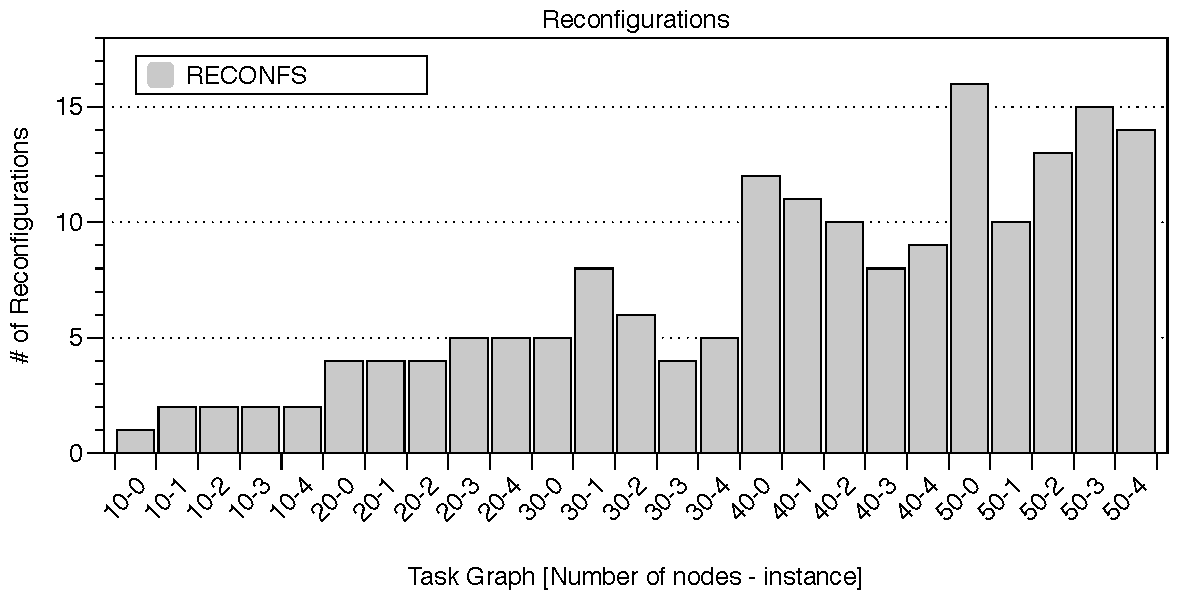
\includegraphics[width=\textwidth]{./capitoli/figure/cap6/FPL_Reconfs.pdf}
  \caption{Numero di riconfigurazioni eseguite per ciascun task graph.}
  \label{fig:numeroRiconfigurazioni}
 \end{center}
\end{figure}



\begin{figure}[t]
 \begin{center}
  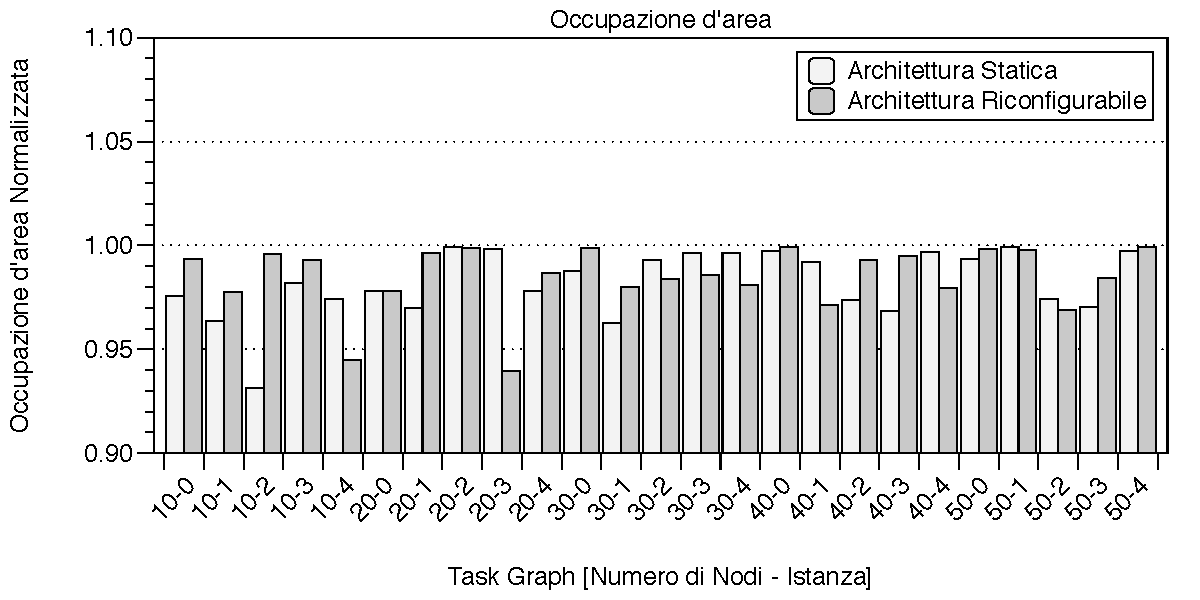
\includegraphics[width=\textwidth]{./capitoli/figure/cap6/FPL_Area.pdf}
  \caption{Uso dell'area, normalizzato rispetto all'area totale.}
  \label{fig:usoArea}
 \end{center}
\end{figure}

\paragraph{Area utilizzata}
La figura \ref{fig:usoArea} rappresenta l'utilizzo dell'area
riconfigurabile da parte di MapR, relativo al mapping migliore trovato durante
l'esplorazione. L'area occupata dai mapping \`e normalizzata rispetto all'area totale.
Si pu\`o vedere dalla figura come in quasi tutti i casi l'area occupata sia
circa uguale all'area disponibile sul dispositivo, senza che si verifichino
violazioni di vincoli.



\subsection{Confronto a runtime}
Per ciascun task graph utilizzato negli esperimenti sullo speedup rispetto alla baseline software
e sul mapping dei task, \`e stato generato un runtime manager che gestisca lo scheduling dei task \cite{DurelliRuntimeManager},
seguendo le indicazioni dello scheduler, in particolare la fase di postprocessing, vista nella sezione
\ref{subsec:fasePostprocessing}, in cui viene esplicitato l'ordine di scheduling dei task.

Per la validazione del runtime manager e l'analisi degli overhead introdotti rispetto alle stime
illustrate nelle precedenti sezioni, sono stati realizzati dei core che implementano un contatore
configurabile (per modellizzare il tempo di esecuzione dei task). I core sono stati creati utilizzando
\emph{Vivado HLS} \cite{VivadoHLS}, i loro requisiti in termini di risorse riflettono quanto
specificato dai task graph creati tramite \ac{TGFF}.

Il sistema finale \`e stato realizzato connettendo manualmente i core generati con Vivado HLS,
l'architettura target \`e una scheda ZedBoard con chip xc7z020-clg484, prodotto da Xilinx
\cite{XilinxZC702}. Il chip sopraccitato \`e composto da un processore general-purpose dual-core
ARM Cortex A9, e da una porzione di logica riconfigurabile collegata al processore.
Il processore, che esegue il kernel di \emph{PetaLinux},\footnote{PetaLinux \`e una distribuzione
Linux specifica per lo sviluppo e la progettazione di sistemi embedded.} gestisce
sia il runtime manager che i task dell'applicazione mappati su implementazioni software;
la logica riconfigurabile \`e invece dedicata ai task con implementazioni hardware.

\paragraph{Risultati ottenuti}
I tempi di esecuzione relativi a ciascuna istanza di task graph sono stati raccolti e confrontati
con le stime fornite al termine dell'esplorazione da MapR, allo scopo di rilevare l'overhead
introdotto dalla gestione a runtime dell'applicazione; i risultati del confronto sono
rappresentati in figura \ref{fig:speedupBaselineRuntime}.
Come si pu\`o vedere dalla figura, gli speedup ottenuti sono diversi rispetto alle stime
illustrate in figura \ref{fig:speedupBaseline}, tuttavia la distribuzione seguita \`e la stessa;
questo perch\`e in fase di esplorazione MapR ha a disposizione le stime dei tempi di esecuzione
dei task e delle riconfigurazioni, ma non \`e fornita nessuna informazione riguardo gli overhead
introdotti dal meccanismo che gestisce l'esecuzione dell'applicazione sul dispositivo, a runtime.
La soluzione ottenuta con il template riconfigurabile \`e comunque migliore, ma per istanze
con un elevato numero di nodi gli speedup decrescono da $2\text{x}$ a $1,25\text{x}$ rispetto alla
baseline software.

In generale, pur migliorando la gestione a runtime e riducendo gli overhead introdotti da questa,
non ci si pu\`o aspettare che i risultati stimati in fase di esplorazione siano uguali a quelli ottenuti
dall'effettiva esecuzione sul dispositivo; i risultati ottenuti in fase di esplorazione rappresentano quindi
un limite superiore al miglioramento delle performance che si pu\`o ottenere, il designer ha comunque il compito
di valutare l'effettivo speedup introdotto.

\begin{figure}[b]
 \begin{center}
  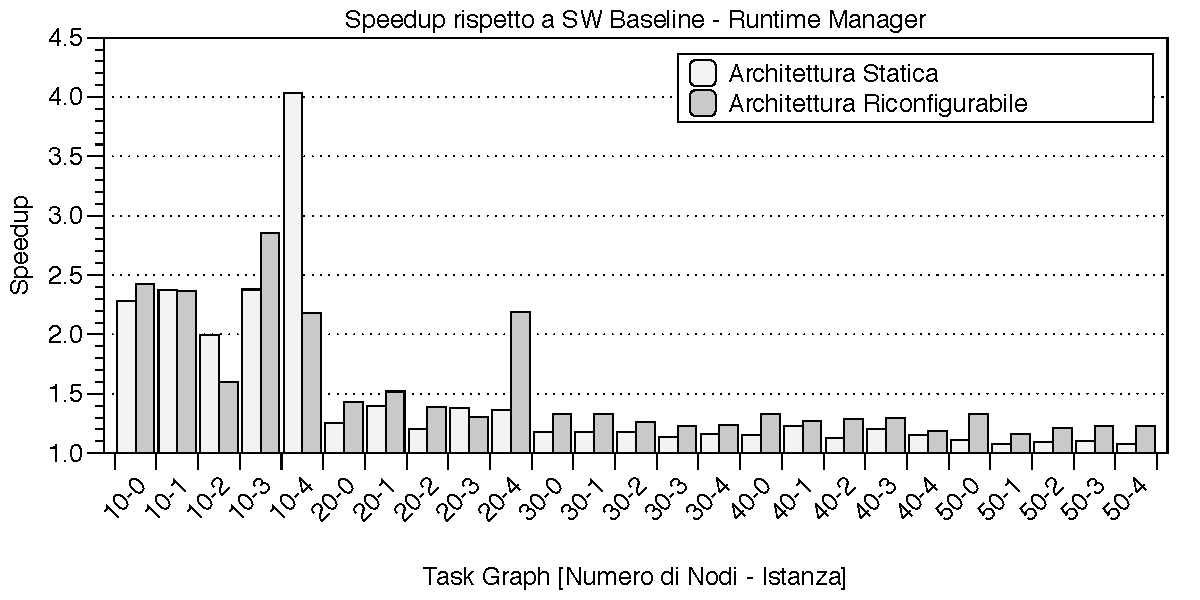
\includegraphics[width=\textwidth]{./capitoli/figure/cap6/FPL_Runtime.pdf}
  \caption{Speedup dell'architettura statica e riconfigurabile rispetto alla
  baseline software, dopo l'esecuzione sul dispositivo.}
  \label{fig:speedupBaselineRuntime}
 \end{center}
\end{figure}

